% !TEX TS-program = pdflatexmk
\documentclass[12pt]{article}

% Layout.
\usepackage[top=1in, bottom=0.75in, left=1in, right=1in, headheight=1in, headsep=6pt]{geometry}

% Fonts.
\usepackage{mathptmx}
\usepackage[scaled=0.86]{helvet}
\renewcommand{\emph}[1]{\textsf{\textbf{#1}}}
\newcommand{\ans}[1][1in]{\rule{#1}{.5pt}}

\usepackage[parfill]{parskip}

% Misc packages.
\usepackage{amsmath,amssymb,latexsym}
\usepackage{graphicx,hyperref}
\usepackage{array}
\usepackage{xcolor}
\usepackage{multicol,tikz}
\usetikzlibrary{calc, positioning}
\usepackage{tabularx,colortbl,booktabs,xparse}
\usepackage{enumitem}

% Rotation: \rot[<angle>][<width>]{<stuff>}
\NewDocumentCommand{\rot}{O{45} O{1em} m}{\makebox[#2][l]{\rotatebox{#1}{#3}}}%

\usepackage{fancyhdr}
\pagestyle{fancy} 
\lhead{\large\sf\textbf{MATH F113X: Graph Theory Intro}}
%\chead{\large\sf\textbf{lecture notes}}
%\rhead{\large\sf\textbf{Day 1}}

\begin{document}
\begin{enumerate}
\item \emph{Example:} Some cities in Alaska
\begin{center}
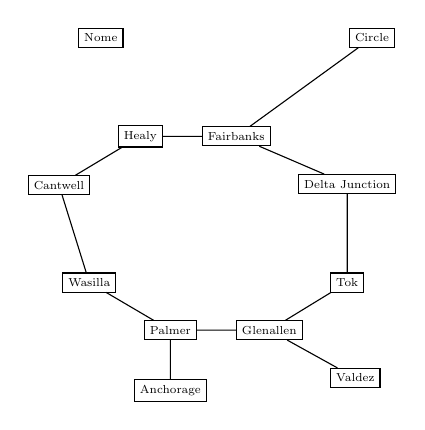
\begin{tikzpicture}[city/.style = {draw, font = \scriptsize, scale = .6}]
\node[city] (fai) at (2,0) {Fairbanks};
\node[city, above right= of fai] (cir) {Circle};
\node[city, below right = .5 of fai] (delta) {Delta Junction};
\node[city, below = of delta] (tok) {Tok};
\node[city, below left = .5 of tok] (glen) {Glenallen};
\node[city, below right = .5 of glen] (valdez) {Valdez};
\node[city, left = .5 of glen] (palmer) {Palmer};
\node[city, below = .5 of palmer] (anc) {Anchorage};
\node[city, above left = .5 of palmer] (was) {Wasilla};
\node[city,  left = .5  of fai] (healy) {Healy};
\node[city, below left = .5 of healy](cant) {Cantwell};
\node[city, above left = of fai] (nome) {Nome};
\draw (fai) -- (cir);
\draw (fai) -- (delta) -- (tok) -- (glen) -- (palmer) -- (was) -- (cant) -- (healy) -- (fai);
\draw (glen) -- (valdez);
\draw (palmer) -- (anc);
\end{tikzpicture}
\end{center}
%\begin{enumerate}
\item \emph{vertex} (plural: vertices), \emph{edge, graph}; ways to represent graphs
	
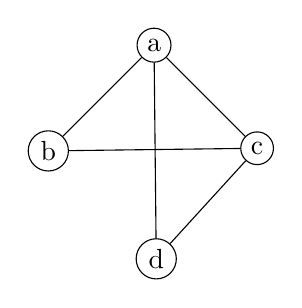
\begin{tikzpicture}[vtx/.style={draw, circle, inner sep = 2 pt}]
\node[vtx] (1) {a};
\node[vtx, below left = of 1] (2) {b};
\node[vtx, below right = of 1] (3) {c};
\node[vtx, below right = of 2] (4) {d};
\draw (1) -- (2) -- (3) -- (4) -- (1);
\draw(1) -- (3);
\end{tikzpicture}

\vfill
	
\item \emph{Example:} Vertices are \emph{classes}. What might edges represent?
\vfill	
		
\newpage

\item  \emph{Degree} of a vertex

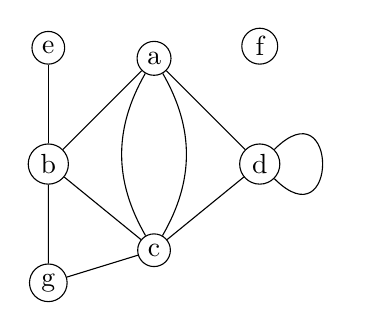
\begin{tikzpicture}[vtx/.style={draw, circle, inner sep = 2 pt}]
\node[vtx] (1) at (0,0) {a};
\node[vtx, below left = of 1] (2) {b};
\node[vtx, below  = 2 of 1] (3) {c};
\node[vtx, below right  = of 1] (4) {d};
\node[vtx, above  = of 2] (5) {e};
\node[vtx, above = of 4] (6) {f};
\node[vtx, below = of 2] (7) {g};
\draw (1) -- (2) -- (3) -- (4) -- (1);
\draw (1) to[bend left = 30] (3);
\draw (1) to[bend right = 30] (3);
\draw (4) to[out = -45, in = 45, looseness = 8] (4);
\draw (2) -- (5);
\draw (3) -- (7) -- (2);
\end{tikzpicture}

\vfill

\item \emph{Path} in a graph

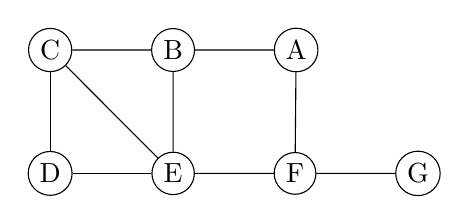
\begin{tikzpicture}[vtx/.style={draw, circle, inner sep = 2 pt}]
\node[vtx] (A) at (0,0) {A};
\node[vtx, left = of A] (B) {B};
\node[vtx, left = of B] (C) {C};
\node[vtx, below = of C] (D) {D};
\node[vtx, right = of D] (E) {E};
\node[vtx, right = of E] (F) {F};
\node[vtx, right = of F] (G) {G};
\draw (A) -- (B) -- (C) -- (E) -- (F) -- (G);
\draw (A) -- (F);
\draw (E) -- (F);
\draw (B) -- (E);
\draw (C) -- (D) -- (E);
\end{tikzpicture}

\vfill

\item A graph is \emph{connected} if...

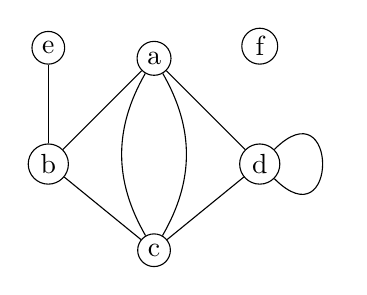
\begin{tikzpicture}[vtx/.style={draw, circle, inner sep = 2 pt}]
\node[vtx] (1) at (0,0) {a};
\node[vtx, below left = of 1] (2) {b};
\node[vtx, below  = 2 of 1] (3) {c};
\node[vtx, below right  = of 1] (4) {d};
\node[vtx, above  = of 2] (5) {e};
\node[vtx, above = of 4] (6) {f};
\draw (1) -- (2) -- (3) -- (4) -- (1);
\draw (1) to[bend left = 30] (3);
\draw (1) to[bend right = 30] (3);
\draw (4) to[out = -45, in = 45, looseness = 8] (4);
\draw (2) -- (5);
\end{tikzpicture}

\vfill

\item A \emph{circuit} in a graph...

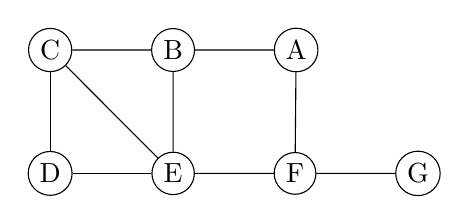
\begin{tikzpicture}[vtx/.style={draw, circle, inner sep = 2 pt}]
\node[vtx] (A) at (0,0) {A};
\node[vtx, left = of A] (B) {B};
\node[vtx, left = of B] (C) {C};
\node[vtx, below = of C] (D) {D};
\node[vtx, right = of D] (E) {E};
\node[vtx, right = of E] (F) {F};
\node[vtx, right = of F] (G) {G};
\draw (A) -- (B) -- (C) -- (E) -- (F) -- (G);
\draw (A) -- (F);
\draw (E) -- (F);
\draw (B) -- (E);
\draw (C) -- (D) -- (E);
\end{tikzpicture}

\vfill
\end{enumerate}
\end{document}